\section*{Optimal $\beta$ obtaining}



\subsection*{For Unregularised Linear Regression}
In linear regression, the loss function is defined as:
$$
    RSS(\beta)=\sum_{i=1}^N(y_i-\hat{y}_i)^2=\sum_{i=1}^N(y_i-\textbf{X}_i\beta )^2\\
$$
($\beta$ here is the transpose of the $\beta$ in section 2.2; the reason for this is mere simplification).
$$
    RSS(\beta)=(\textbf{y}-\textbf{X}\beta)^T(\textbf{y}-\textbf{X}\beta)
$$
From this, differentiating with respect to $\beta$, we can get the normal equation:
$$
\textbf{X}^T(\textbf{y}-\textbf{X}\beta)=0
$$
And solving for $\beta$:
\begin{equation}
    \beta=(\textbf{X}^T\textbf{X})^{-1}\textbf{X}^T\textbf{y}
\end{equation}
\subsection*{For Regularised Ridge}
In ridge regression, the loss function is defined as:
$$
 RSS(\beta)=(\textbf{y}-\textbf{X}\beta)^T(\textbf{y}-\textbf{X}\beta)+\alpha\beta^T\beta
$$
As in linear regression, differentiating with respect to $\beta$ and equalling to zero:
$$
\textbf{X}^T(\textbf{y}-\textbf{X}\beta)+\alpha\beta=0
$$
And solving for $\beta$:
$$
\beta=(\textbf{X}^T\textbf{X}+\alpha\mathbb{1})^{-1}\textbf{X}^T\textbf{y}
$$
where,
\begin{equation}
   \mathbb{1} =
    \begin{pmatrix}
0 & 0 & 0 & \cdots & 0\\
0 & 1 & 0 & \cdots & 0\\
0 & 0 & 1 & \cdots & 0\\
\vdots & \vdots & \vdots & \ddots & \vdots\\
0 & 0 & 0 & \cdots & 1
\end{pmatrix}_{N \times N}
\end{equation}
and N is the number of descriptor features.

\section*{Features}
Here, you can find the description of the top 10 features contemplated. These were considered according to the significance with respect to the meaning of the task, and according to the times they were selected in nested cross-validation feature selection algorithm for Random Forest (Figure 4.4).

\begin{figure}[h]
    \centering
    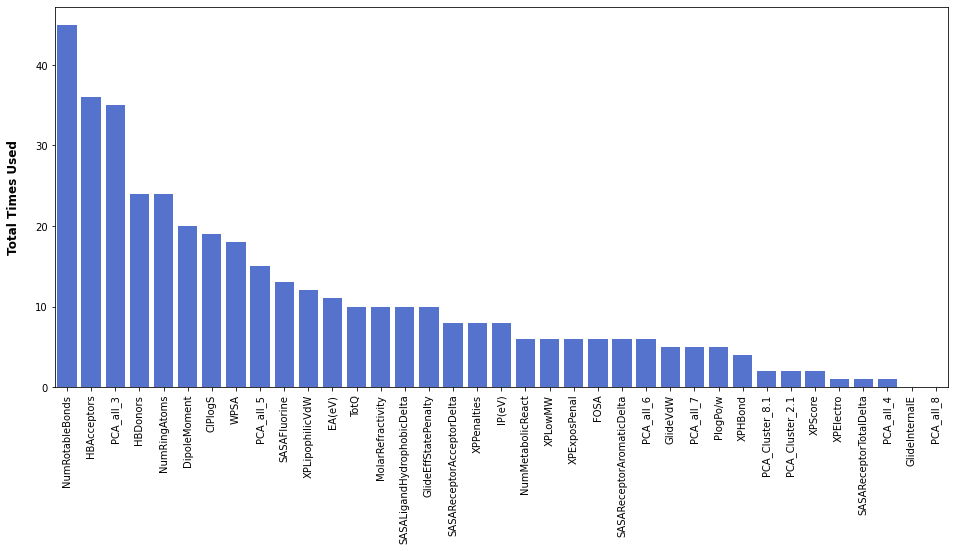
\includegraphics[width=\textwidth]{Images/Appendix/Features.png}
    \caption{Most important features according to the feature selection algorithm and the times used in constructing the Random Forest model.}
\end{figure}
\textbullet\hspace{0.5cm}\textbf{NumRotableBonds}.The number of rotable bonds is a very significant chemical feature as it describes the structural flexibility of the ligand. Molecules with a larger number of rotable bonds tend to have a wider variety of stable structures and thus more ways in which they can bind to the receptor, but at the same time these bound structures can have much higher energy compared to their minimum energy structure, which can result in the bound structure being energetically unfavourable.\\\\
\textbullet\hspace{0.5cm}\textbf{HBAcceptors/HBDonors}. The number of atoms in the ligand that can act as acceptors/donors in a hydrogen bond. The higher this number, the more likely that a hydrogen bond between the ligand and the receptor or a water molecule is formed, which is one of the most common ways in which ligands bind to protein receptors.\\\\
\textbullet\hspace{0.5cm}\textbf{NumRingAtoms}. The number of atoms that belong to an aromatic ring. The larger this number, the more aromatic the ligand, meaning that the ligand is more likely to be stable in hydrophobic environments, where aromatic rings stabilize through the formation of hydrophobic interactions such as $\pi$-stacking.\\\\
\textbullet\hspace{0.5cm}\textbf{DipoleMoment}.The dipole moment of the ligand. The polarization induced by the electric fields generated by the receptor is known to be very important in understanding the binding mechanism of a large amount of ligands.\\\\
\textbullet\hspace{0.5cm}\textbf{CIPlogS}. The aqueous solubility of the ligand. It can be understood as a measure of the hydrophilicity of the ligand, $i.e.$, the higher the solubility, the more likely the ligand is stable in conformations where it is highly exposed to water molecules.\\\\
\textbullet\hspace{0.5cm}\textbf{WPSA and SASAFluorine}. Measure of the surface area of the molecule containing polar or weakly polar atoms (halogens, P, S, and F). Ligands with a high amount of polar atoms tend to be stable in binding pockets containing a high amount of polar amino acids.\\\\
\textbullet\hspace{0.5cm}\textbf{XPElectro}. Measures the energy associated with the electrostatic interactions between the ligand and the receptor in the bound conformation. Conformations where these interactions are stronger should, in principle, be more stable.\\\\
\textbullet\hspace{0.5cm}\textbf{EA(eV)}. Electron affinity of the ligand.\\\\


\section*{Grid Search Eligibility Counts}
The examined sections for grid search  yielded different values for the optimal values of the hyperparameters.

\subsection*{Ridge}

\begin{figure}[h!]
    \centering
    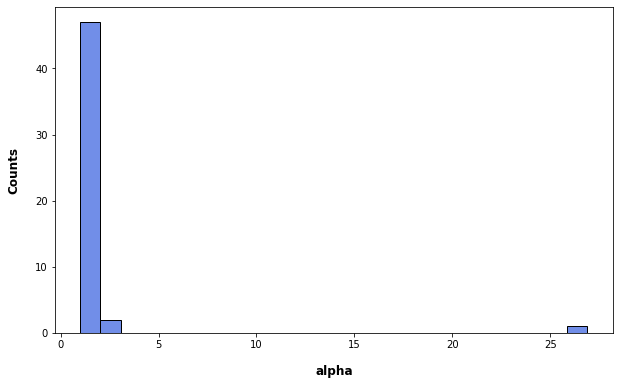
\includegraphics[width=0.6\textwidth]{Images/Appendix/CountsRidge.png}
    \caption{Grid search counts for ridge regression. Optimal value for regularisation parameter $\alpha=1$.}
\end{figure}
\newpage

\subsection*{Random Forest}

\begin{figure}[h!]
    \centering
    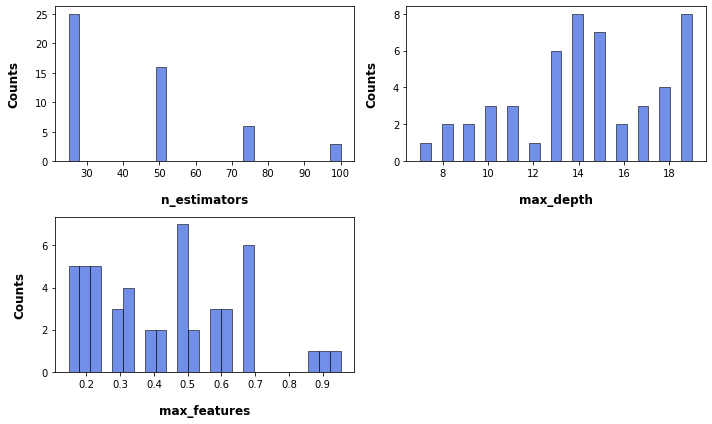
\includegraphics[width=\textwidth]{Images/Appendix/Counts.png}
    \caption{Grid search counts for Random Forest. As it can be observed, the grid search gave a fairly homogeneous distribution for the maximum depth and ratio of features, while the optimal value for the number of trees was about 25.}
\end{figure}
